
\documentclass[11pt]{article}

\usepackage{amsmath,amssymb}
\usepackage{booktabs}
\usepackage{graphicx}
\usepackage[hyphens]{url}
\usepackage{hyperref}
\usepackage[margin=1in]{geometry}
\usepackage[numbers,sort&compress]{natbib}
\usepackage{xcolor}
\usepackage{array}
\usepackage{enumitem}
\usepackage[affil-it]{authblk}

\renewcommand{\arraystretch}{1.3}

\newcommand{\todo}[1]{\textcolor{red}{[TODO: #1]}}

\title{A Composition-Controlled Evaluation of RNA Structure\\
Awareness in Foundation Models}

\author{Elliot Tower}
\affil{Independent researcher \\ \texttt{elliot@elliottower.ai}}
\date{}

\begin{document}
\maketitle

\begin{abstract}
RNA foundation models are entering drug-discovery pipelines, where their
structural confidence scores guide target selection for screening campaigns.
Systematic controls separating learned RNA structure from nucleotide
composition and architectural inductive bias are largely absent from current
evaluations. We present a pre-registered, composition-controlled
evaluation of seven RNA and DNA foundation models across 16 therapeutic RNA
targets spanning eight druggable positives, five non-druggable negatives, and
three graded HTT repeat-length controls. The evaluation applies a two-stage
gate: Stage~1 tests whether each model's mutation sensitivity exceeds a
nucleotide-stratified permutation null (1,000 permutations, 95th-percentile
threshold); Stage~2 tests whether the model's best-head attention pattern
correlates with the ViennaRNA-predicted contact map ($\rho_S \geq 0.10$).
The primary pre-registered hypothesis---that the gate
discriminates druggable from non-druggable targets better than probing
accuracy---fails ($p = 1.0$): the composition null rejects 14--16 of 16
targets per model, including most positives. The gate catches a distinct
failure mode the primary hypothesis did not target: two targets pass the
composition null but lack attention-contact correspondence (the ``degeneracy
trap''). A five-seed untrained-weight control reveals that Nucleotide
Transformer v2 produces identical attention-contact correlation from random
weights (delta $= -0.002$, 95\% CI $[-0.011, +0.007]$), exposing a purely
architectural artifact invisible to any evaluation that omits untrained
controls. The composition-null gate functions as an artifact detector rather
than a druggability predictor---a role that existing RNA foundation model
evaluations do not fill.
\end{abstract}

\paragraph*{Author summary}
RNA foundation models are increasingly used to prioritize drug targets:
a model assigns a confidence score to a candidate RNA, and that score
determines whether the target advances to expensive experimental
screening.  We tested whether these scores reflect genuine structural
understanding or simpler confounds.  Using a panel of 16 therapeutic RNA
targets with known druggability status, we found that most models'
sensitivity to mutations can be explained by nucleotide composition
alone---the models respond differently to mutations at stem positions
than loop positions, but so would any model that has learned which
nucleotides tend to appear in stems.  A separate control revealed that
one model's attention patterns correlate with RNA structure even when its
weights are completely random, an architectural artifact rather than
learned knowledge.  These findings suggest that per-target composition
controls and untrained-weight baselines should be standard in RNA
foundation model evaluations.  All hypotheses were pre-registered before
any data were analyzed.


%% ======================================================================
\section{Introduction}
%% ======================================================================

RNA foundation models trained on millions of non-coding RNA sequences have
achieved strong performance on secondary-structure prediction benchmarks and
are now entering therapeutic target-selection pipelines~\citep{rnafm2022,
rinalmo2024, ernierna2024, atomicai2025, alnylam2026}. A model's structural
confidence score on a candidate RNA target increasingly determines whether
that target proceeds to experimental screening---a decision that commits
hundreds of thousands of dollars in assay development and compound library
costs. Whether a high confidence score reflects learned RNA structure or a
confound that mimics it has received limited systematic evaluation.

Two confounds dominate. Stem regions in RNA secondary structures are enriched
for G and C (mean GC content $\sim$68.5\%) relative to loop regions
($\sim$43.9\%)~\citep{towerC2026}. A model that has learned to respond to
local GC content will show high mutation sensitivity at stem positions and
low sensitivity at loop positions---the same pattern as genuine structural
awareness---without encoding base-pairing geometry. A nucleotide-stratified
permutation null, which shuffles stem and loop labels within each nucleotide
type, controls for this confound: in a prior evaluation across 52 Rfam
families, RNA-FM's apparent structure sensitivity ratio dropped from
$\sim$5.5$\times$ to $1.8\times$ after nucleotide control, and no family
survived both nucleotide and dinucleotide nulls~\citep{towerC2026}. A second,
independent confound is architectural inductive bias: transformer attention
patterns can correlate with RNA contact maps through positional encoding
alone, independent of learned weights, a failure mode invisible to
evaluations that test only trained models.

Existing evaluations do not control for either confound at the per-target
level. OmniGenome~\citep{omnigenome2024} and CHANRG~\citep{chanrg2026}
evaluate aggregate accuracy across held-out families---answering whether a
model generalizes to new sequences, not whether its confidence on a specific
therapeutic target is real. A model can achieve 78\% aggregate probing
accuracy while passing a composition null on only 1 of 16 targets.

We present a pre-registered, per-target evaluation of seven foundation
models (five RNA, two DNA) against 16 therapeutic RNA targets with known
druggability status, applying a two-stage composition-controlled gate and an
untrained-weight architectural control. Four hypotheses were pre-registered
and frozen with SHA-256 hashes before evaluation. The primary
hypothesis---that the gate discriminates druggable from non-druggable
targets---fails. The gate catches composition artifacts and architectural
degeneracy that no existing evaluation detects, functioning as a quality
filter on computational evidence rather than a druggability predictor.


%% ======================================================================
\section{Methods}
%% ======================================================================

Figure~\ref{fig:schematic} summarizes the two-stage gate and
untrained-weight control.

\begin{figure}[htbp]
\centering
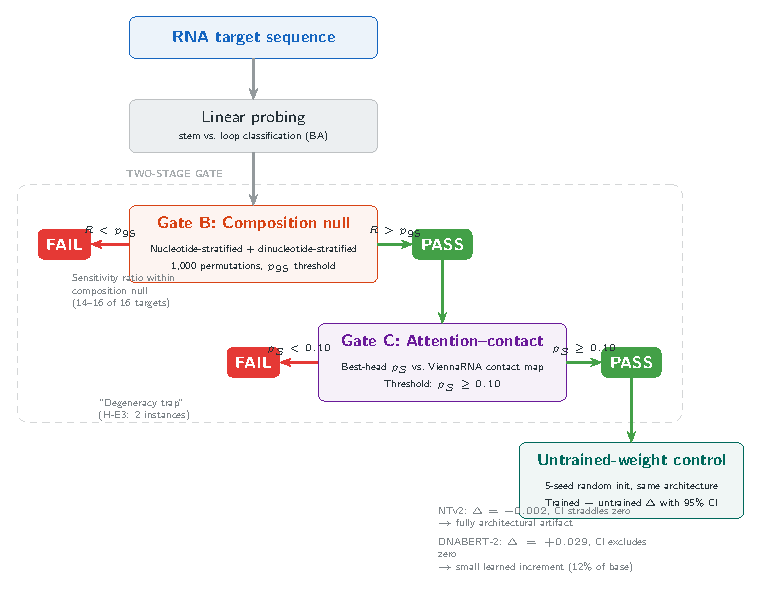
\includegraphics[width=0.85\textwidth]{figures/figure1_gate_schematic.pdf}
\caption{Two-stage composition-controlled evaluation pipeline. Gate~B tests
whether each model's mutation sensitivity ratio exceeds a
nucleotide-stratified and dinucleotide-stratified permutation null (1,000
permutations, 95th-percentile threshold). Targets surviving Gate~B proceed
to Gate~C, which tests attention--contact correspondence ($\rho_S \geq
0.10$). Targets passing Gate~B but failing Gate~C fall into the
``degeneracy trap'' (H-E3). The untrained-weight control re-runs Gate~C
with randomly initialized weights to separate learned representations from
architectural inductive bias.}
\label{fig:schematic}
\end{figure}

\subsection{Target benchmark}

Sixteen RNA targets were selected to span three categories: eight positives
(POS-01 through POS-08) with established druggability evidence, five
negatives (NEG-01 through NEG-05) with no known druggability, and three
graded controls (CTL-01 through CTL-03) consisting of HTT exon~1 CAG-repeat
constructs at lengths 17, 36, and 60, providing a monotonicity test for
repeat-length sensitivity. Table~\ref{tab:targets} lists each target with
its RNA type, sequence length, and druggability evidence. The benchmark is
stored as \texttt{druggability\_benchmark\_v2.tsv} and was frozen before
evaluation.

\begin{table}[htbp]
\centering
\caption{Target benchmark. POS: druggable positive; NEG: non-druggable
negative; CTL: graded HTT repeat-length control. Druggability evidence lists
published ligands or structural rationale. Synthetic controls (NEG-04,
NEG-05) are generated at runtime with frozen RNG seeds.}
\label{tab:targets}
\small
\begin{tabular}{llllrl}
\toprule
\textbf{ID} & \textbf{Target} & \textbf{RNA type} & \textbf{Source} & \textbf{nt} & \textbf{Evidence} \\
\midrule
POS-01 & SMN2 exon 7 splice element & pre-mRNA & NM\_017411.3 & 54 & Risdiplam (FDA) \\
POS-02 & FMN riboswitch aptamer & riboswitch & RF00050 & 78 & Ribocil ($K_d$ 16~nM) \\
POS-03 & HCV IRES domain II & viral IRES & PDB 1P5O & 77 & Cpd 13 ($K_d$ 720~nM) \\
POS-04 & HIV-1 TAR apical loop & viral element & PDB 1ARJ & 29 & Amiloride derivatives \\
POS-05 & PreQ1 riboswitch aptamer & riboswitch & RF00522 & 51 & Cpd 1 ($K_d$ 99~nM) \\
POS-06 & MALAT1 ENE triple helix & lncRNA & PDB 4PLX & 76 & Triplex stabilizers \\
POS-07 & EV71 IRES stem-loop II & viral IRES & PDB 6XB7 & 41 & DMA-135 ($K_d$ 500~nM) \\
POS-08 & SARS-CoV-2 5$'$ UTR SL & viral element & NC\_045512.2 & 47 & DMA-155 (IC$_{50}$ 10~$\mu$M) \\
\midrule
NEG-01 & HOTAIR lncRNA domain 1 & lncRNA & NR\_047517.1 & 100 & R-scape: no covariation \\
NEG-02 & SRA lncRNA 5$'$ region & lncRNA & NR\_045587.1 & 100 & R-scape: no covariation \\
NEG-03 & Xist repeat A tandem & lncRNA & NR\_001564.2 & 111 & No conserved structure \\
NEG-04 & Shuffled tRNA-Phe & synthetic & seed 42 & 76 & Dinuc-preserved shuffle \\
NEG-05 & Random GC-matched & synthetic & seed frozen & 76 & No designed structure \\
\midrule
CTL-01 & HTT CAG17 (normal) & mRNA repeat & NM\_002111.7 & 235 & Repeat-length ref \\
CTL-02 & HTT CAG36 (threshold) & mRNA repeat & NM\_002111.7 & 292 & Repeat-length ref \\
CTL-03 & HTT CAG60 (severe) & mRNA repeat & NM\_002111.7 & 364 & Repeat-length ref \\
\bottomrule
\end{tabular}
\end{table}

\subsection{Foundation model panel}

Seven models were evaluated: RNA-FM~\citep{rnafm2022},
RiNALMo~\citep{rinalmo2024}, ERNIE-RNA~\citep{ernierna2024},
SpliceBERT~\citep{splicebert2024}, UTR-LM~\citep{utrlm2024},
Nucleotide Transformer v2 (NTv2)~\citep{ntv22023}, and
DNABERT-2~\citep{dnabert22024}. Five are RNA models; NTv2 and DNABERT-2 are
DNA models included to test cross-domain transfer. All models were used with
frozen pretrained weights (no fine-tuning). DNABERT-2's BPE tokenization
prevents nucleotide-level mutation mapping, so it is excluded from Gate~B
(composition-null sensitivity) and included only in Gate~C
(attention-contact) and probing analyses. For DNABERT-2, BPE token-level
hidden states were expanded to nucleotide resolution via proportional mapping
(\texttt{\_expand\_bpe\_to\_nucleotide}), and attention was aggregated to
nucleotide-level contacts (\texttt{\_aggregate\_contacts\_to\_tokens}) using
a 6-mer approximation. Table~\ref{tab:models} summarizes the model panel.

\begin{table}[htbp]
\centering
\caption{Foundation model panel. Token resolution determines Gate~B
eligibility: DNABERT-2's BPE tokenization prevents nucleotide-level
mutation mapping.}
\label{tab:models}
\small
\begin{tabular}{llrrl}
\toprule
\textbf{Model} & \textbf{Architecture} & \textbf{$d$} & \textbf{Layers} & \textbf{Token res.} \\
\midrule
RNA-FM~\citep{rnafm2022}       & Transformer encoder  & 640 & 12 & nucleotide \\
RiNALMo~\citep{rinalmo2024}    & Transformer encoder  & 1280 & 33 & nucleotide \\
ERNIE-RNA~\citep{ernierna2024}  & Transformer encoder  & 768 & 12 & nucleotide \\
SpliceBERT~\citep{splicebert2024} & BERT              & 512 & 6 & nucleotide \\
UTR-LM~\citep{utrlm2024}       & Transformer encoder  & 128 & 6 & nucleotide \\
NTv2~\citep{ntv22023}           & ESM (attn + GLU)     & 512 & 12 & 6-mer \\
DNABERT-2~\citep{dnabert22024}  & MosaicBERT           & 768 & 12 & BPE \\
\bottomrule
\end{tabular}
\end{table}

\subsection{Probing accuracy}

For each model--target pair, a linear probe was trained on per-position
embeddings (extracted at each model layer) to classify nucleotide positions
as stem or loop, using the ViennaRNA-predicted secondary structure as ground
truth. Balanced accuracy (BA) = (sensitivity + specificity) / 2 was computed
across all positions in all 16 targets, and the best-layer BA was reported
per model.

\subsection{Gate B: composition-null mutation sensitivity}

Each nucleotide position in a target sequence was perturbed by complement
swap (A$\leftrightarrow$U, C$\leftrightarrow$G, with T treated as equivalent
to U for DNA models). The model embedding distance (L2 norm) between
wild-type and perturbed sequence was measured at the mutated position,
extracted at each model layer. The structure sensitivity ratio $R$ was
computed as the ratio of mean embedding distance at stem positions to mean
distance at loop positions, maximized across layers:

\begin{equation}
R = \max_{\ell} \frac{\bar{d}_{\text{stem}}^{(\ell)}}{\bar{d}_{\text{loop}}^{(\ell)}}
\end{equation}

Two null distributions were constructed per target. The
\emph{nucleotide-stratified null} shuffled stem/loop labels independently
within each nucleotide type (A, U, C, G), preserving the compositional
correlation between nucleotide identity and structural role. The
\emph{dinucleotide-stratified null} further conditioned on the identity of
each position's nearest neighbor, controlling for second-order sequence
context. Each null was sampled 1,000 times, with a deterministic per-target
RNG seed (\texttt{42 + rna\_idx $\times$ 1000}). A target passed Gate~B only
if $R$ exceeded the 95th percentile of \emph{both} null distributions.

\subsection{Gate C: attention-contact correspondence}

For each model--target pair, per-head attention matrices were extracted at
each layer. Each attention head's matrix was compared to a binary contact
matrix derived from ViennaRNA RNAfold~2.7.0 (37°C, dangles~2, Turner
2004~\citep{lorenz2011}) via Spearman rank correlation. The best-head
correlation $\rho_S$ (maximum across all layers and heads) was recorded per
model--target pair. A target passed Gate~C if $\rho_S \geq 0.10$, a
threshold set from noise-floor considerations: for sequences of length
100--400, the standard error of $\rho_S$ under the null is 0.05--0.10.

\subsection{Untrained-weight control}

To distinguish learned structural representations from architectural
inductive bias, the untrained-weight control re-ran Gate~C with randomly
initialized weights. For each model, pretrained weights were loaded to
establish the architecture (layer count, hidden size, intermediate size),
then all weight tensors were reinitialized: Xavier uniform for 2D weight
matrices, ones for LayerNorm scale, zeros for biases. This preserves
positional encodings and attention geometry while removing all learned
representations. A five-seed sweep (seeds 0--4, \texttt{torch.manual\_seed}
before reinitialization) quantified initialization variance. The pretrained
minus untrained delta on mean $\rho_S$ across targets was computed with a
95\% confidence interval using $t(4, 0.025) = 2.776$.

The control was applied to the two DNA models (NTv2 and DNABERT-2) because
both showed 16/16 Gate~C pass rates, including on negative controls---a
pattern suggesting architectural origin. RNA models showed lower and more
variable Gate~C pass rates, consistent with target-specific learned
representations.

\subsection{Pre-registered hypotheses}

Four hypotheses were specified in the pre-registration document
(\texttt{preregistration\_E1\_druggability\_gate\_v3.md}) and frozen with
SHA-256 hash before evaluation:

\begin{enumerate}[label=\textbf{H-E\arabic*}]
\item \textbf{(Primary)} Gate BA $>$ probing BA with $\geq 0.10$ margin,
  tested via Wilcoxon signed-rank on 6 model-level paired differences
  (one-sided, $\alpha = 0.05$). DNABERT-2 excluded.
\item Gate-passing models show Spearman $\rho \geq 0.8$ between embedding
  distance and HTT repeat length (CTL-01/02/03); gate-failing models show
  $|\rho| < 0.3$.
\item At least one target passes Gate~B but fails Gate~C (demonstrating the
  ``degeneracy trap''---composition-null survival without structural
  correspondence).
\item On negative targets, the gate's rejection rate exceeds probing's
  rejection rate.
\end{enumerate}

\subsection{Implementation}

All experiments ran on NVIDIA A10G GPUs (24~GB VRAM), one model per
container. The full 7-model panel with 1,000 permutations completed in
under 60 minutes wall-clock time. Code, pre-registration documents,
and all result files are available at
\url{https://github.com/elliottower/rna-fm-composition-null}.


%% ======================================================================
\section{Results}
%% ======================================================================

\subsection{Probing accuracy}

All seven models exceed chance on stem-versus-loop classification
(Figure~\ref{fig:results}D; Wilcoxon
signed-rank, $H_0$: median BA $= 0.5$; $W = 28.0$, $p = 0.008$, $n = 7$).
Mean BA across models is 0.686 (range 0.574--0.783). RiNALMo (0.783) and
ERNIE-RNA (0.781) are the strongest probes. The two DNA models, NTv2 (0.576)
and DNABERT-2 (0.574), are weakest---consistent with cross-domain transfer
from DNA pretraining to RNA structure.

\subsection{H-E1 (primary): gate discrimination vs.\ probing}

The pre-registration specifies AUC as the discrimination metric. Because the
composition-null gate produces a binary PASS/FAIL at the 95th-percentile
threshold (a single operating point, not a score), AUC cannot be computed.
Balanced accuracy (BA) is the only discrimination metric available at a
single threshold and is used here as the realized operationalization.

Gate~B BA was computed per model as (sensitivity + specificity)~/~2, where
sensitivity = fraction of 8 POS targets passing, specificity = fraction of 5
NEG targets rejected.

\begin{center}
\begin{tabular}{lccccc}
\toprule
\textbf{Model} & \textbf{Sens} & \textbf{Spec} & \textbf{Gate BA} & \textbf{Probing BA} & \textbf{Diff} \\
\midrule
RNA-FM      & 0.000 & 1.000 & 0.500 & 0.625 & $-0.125$ \\
RiNALMo     & 0.125 & 1.000 & 0.562 & 0.783 & $-0.221$ \\
ERNIE-RNA   & 0.125 & 1.000 & 0.562 & 0.781 & $-0.219$ \\
SpliceBERT  & 0.250 & 1.000 & 0.625 & 0.743 & $-0.118$ \\
UTR-LM      & 0.000 & 1.000 & 0.500 & 0.720 & $-0.220$ \\
NTv2        & 0.125 & 0.800 & 0.463 & 0.576 & $-0.114$ \\
\bottomrule
\end{tabular}
\end{center}

All six differences are negative. Wilcoxon signed-rank (one-sided, $H_a$:
gate $>$ probing): $W = 0.0$, $p = 1.000$, $n = 6$. \textbf{H-E1 fails.}
The composition-null gate rejects 14--16 of 16 targets per model
(Figure~\ref{fig:results}A), producing sensitivity of 0.000--0.250 and
making it a worse discriminator than probing on every model. The gate is too stringent to discriminate druggable from
non-druggable targets at $n = 16$.

\subsection{Secondary hypotheses}

\textbf{H-E2} predicts that gate-passing models show Spearman $\rho \geq 0.8$
between embedding distance and HTT repeat length (CTL-01/02/03) while
gate-failing models show $|\rho| < 0.3$. Gate-passing models satisfy the
criterion (4/4, all $\rho = 1.00$), but gate-failing models violate it: both
RNA-FM ($\rho = 0.87$) and UTR-LM ($\rho = 1.00$) show strong monotonicity
despite failing Gate~B. H-E2 fails. Monotonicity is universal---embedding
distance tracks repeat length regardless of gate status, a composition
effect (longer CAG repeats produce more sequence) rather than a learned
structural representation. RNA-FM illustrates this: $\rho = 0.87$ while its
actual distances are numerically zero (CTL-02 $= 0.000$, CTL-03 $= 3 \times
10^{-7}$), a trivial ordering on noise.

\textbf{H-E3} predicts at least one target passes Gate~B but fails
Gate~C---mutation sensitivity exceeding the composition null without
attention-contact correspondence. Two instances were found, both on
SpliceBERT: POS-06 (MALAT1 ENE) and POS-07 (EV71 IRES SLII). H-E3 passes.
These targets survive composition control while the model's attention fails
to correspond to the ViennaRNA-predicted contact map---a screening decision
based on Gate~B alone would accept them.

\textbf{H-E4} predicts that the gate's rejection rate on negatives exceeds
probing's. Gate~B rejects 4--5 of 5 negatives per model (80--100\%), which
trivially exceeds probing's rejection rate under any interpretation. H-E4
is uninformative: Gate~B rejects 80--100\% of everything, so the directional
test is satisfied by blanket stringency rather than selective discrimination.

\begin{figure}[htbp]
\centering
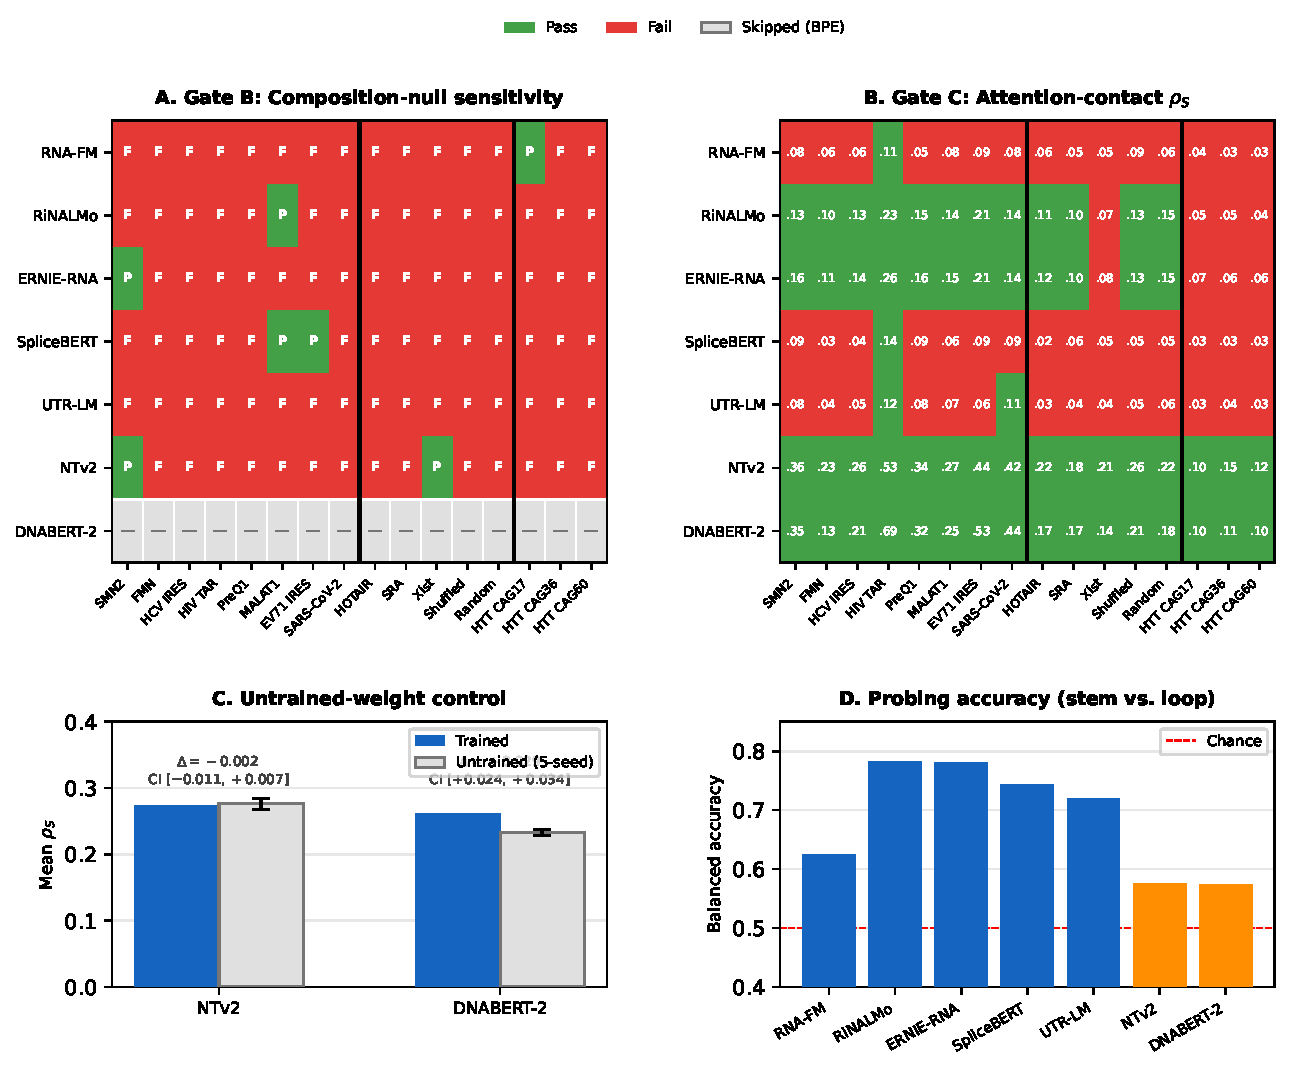
\includegraphics[width=\textwidth]{figures/figure2_results_overview.pdf}
\caption{Results overview. \textbf{A.}~Gate~B (composition-null mutation
sensitivity): most targets fail across all models; DNABERT-2 is excluded
(BPE tokenization). \textbf{B.}~Gate~C (attention--contact $\rho_S$):
NTv2 and DNABERT-2 pass all 16 targets; RNA models show target-specific
variation. Values are best-head Spearman $\rho_S$. \textbf{C.}~Untrained-weight
control: NTv2's attention--contact correlation is fully architectural
($\Delta = -0.002$, CI straddles zero); DNABERT-2 shows a small learned
increment ($\Delta = +0.029$). \textbf{D.}~Probing accuracy (stem vs.\
loop balanced accuracy): all models exceed chance (0.5); RNA models
(blue) outperform DNA models (orange).}
\label{fig:results}
\end{figure}

\subsection{Pre-registered summary}

\begin{center}
\begin{tabular}{lll}
\toprule
\textbf{Hypothesis} & \textbf{Result} & \textbf{Interpretation} \\
\midrule
H-E1 (primary)   & FAIL ($p = 1.0$)    & Probing outperforms gate on all 6 models \\
H-E2              & FAIL                & Monotonicity is universal; gate does not predict it \\
H-E3              & PASS                & Degeneracy trap demonstrated (2 instances) \\
H-E4              & UNINFORMATIVE       & Gate rejects everything; test trivially satisfied \\
\bottomrule
\end{tabular}
\end{center}

The primary hypothesis fails. The composition-null gate with 1,000
permutations and 95th-percentile threshold is too conservative to discriminate
druggable from non-druggable targets at $n = 16$.

\subsection{Architectural artifact in attention-contact correlation}

The untrained-weight control exposes a failure mode orthogonal to the
pre-registered hypotheses (Figure~\ref{fig:results}C). NTv2 passes Gate~C
on all 16 targets (16/16) with trained weights, showing a mean
attention-contact correlation of $\rho_S = 0.274$. With randomly initialized weights, it produces $\rho_S = 0.276 \pm
0.008$ (5-seed mean $\pm$ SD) and passes 16/16 on every seed.

\begin{center}
\begin{tabular}{lcccccc}
\toprule
\textbf{Model} & \textbf{Trained} & \textbf{Untrained} & \textbf{$\Delta$} & \textbf{95\% CI} & \textbf{Trained C} & \textbf{Untrained C} \\
\midrule
NTv2     & 0.274 & 0.276 $\pm$ 0.008 & $-0.002$ & $[-0.011, +0.007]$ & 16/16 & 16/16 \\
DNABERT-2 & 0.262 & 0.233 $\pm$ 0.004 & $+0.029$ & $[+0.024, +0.034]$ & 16/16 & 13--14/16 \\
\bottomrule
\end{tabular}
\end{center}

NTv2's delta is $-0.002$ with a 95\% CI of $[-0.011, +0.007]$, straddling
zero. The ESM-style attention architecture produces structure-correlated
attention from positional encoding alone. The negative control NEG-04
(a dinucleotide-shuffled tRNA with no real secondary structure) scores
$\rho = 0.314$ on untrained NTv2---higher than several positive druggable
targets---confirming that the signal is architectural.

DNABERT-2 shows a statistically detectable learned increment (delta $=
+0.029$, 95\% CI $[+0.024, +0.034]$, excluding zero across all 5 seeds).
The increment is small relative to the untrained baseline: 12\% of the
base $\rho_S = 0.233$. The untrained model already passes 13--14 of 16
targets; training adds at most 2--3 additional passes. The MosaicBERT
architecture produces structure-correlated attention without learned weights;
training adds a detectable layer that rarely changes a gate verdict.

Gate~C does not discriminate druggable from non-druggable targets in either
DNA model. Any evaluation of these models' structural awareness that relies
on attention-contact correlation without an untrained-weight control will
mistake architectural inductive bias for learned representation.


%% ======================================================================
\section{Discussion}
%% ======================================================================

The composition-null gate does not discriminate druggable from non-druggable
RNA targets. This is a pre-registered negative---the hypothesis, test
statistic, and analysis plan were frozen before evaluation---and the negative
is as informative as a positive would have been. At 1,000 permutations with
a 95th-percentile threshold, most models' per-position mutation sensitivity
ratios fall within the range that composition alone predicts. The gate
rejects nearly everything, including most positives. Its value is in a
different role: a target that survives the composition null carries strong
evidence that the model's sensitivity exceeds what nucleotide identity can
explain, and the two SpliceBERT targets that pass Gate~B but fail Gate~C
(H-E3) show that composition-immune sensitivity does not guarantee structural
correspondence. A screening decision based on mutation sensitivity alone
would accept those targets; the two-stage design catches them.

The untrained-weight finding identifies a failure mode orthogonal to
composition. NTv2's attention correlates with RNA contact maps at
$\rho = 0.274$; random weights produce $\rho = 0.276$ (5-seed CI straddling
zero). The ESM-style attention architecture generates structure-correlated
patterns from positional encoding alone. NEG-04, a dinucleotide-shuffled
tRNA with no real secondary structure, scores $\rho = 0.314$ on untrained
NTv2---higher than several positive druggable targets. Any benchmark that
uses attention-contact correlation as evidence of structural learning is
vulnerable to this confound unless it includes an untrained-weight baseline,
a computationally trivial control (one additional forward pass per model).
DNABERT-2 shows a statistically real learned increment ($\Delta = +0.029$,
CI excludes zero across 5 seeds), but the increment is 12\% of the
untrained baseline and changes Gate~C verdicts on at most 2--3 targets. A
continuous metric reporting the pretrained-minus-untrained delta would be
more informative than a binary threshold for models in this regime.

These results have direct consequences for how RNA foundation models are
evaluated. Per-target gating complements aggregate benchmarks: RiNALMo
achieves 78\% probing accuracy while passing Gate~B on 1 of 16 targets.
Aggregate accuracy tells a model developer whether the model has learned
structure in general; per-target gating tells a screening team whether
the model's confidence on their specific target is credible. Composition
control should be standard in mutation sensitivity analyses---the 68.5\%
stem / 43.9\% loop GC asymmetry guarantees that any complement-swap
analysis will show a spurious stem-over-loop ratio unless nucleotide
identity is stratified out.

Several limitations bound the scope of these conclusions. The 16-target
panel constrains statistical power for the primary hypothesis; a larger
panel could establish whether a relaxed threshold or modified null improves
discrimination. The contact-map ground truth derives from ViennaRNA RNAfold,
which may not capture tertiary contacts or context-dependent folds;
experimental structure data (SHAPE-MaP, DMS-MaPseq) would provide more
reliable ground truth. The untrained-weight control was applied only to the
two DNA models; whether architectural artifacts affect RNA-specific
architectures at a detectable level remains open. DNABERT-2's BPE
tokenization makes its absolute $\rho_S$ values non-comparable to
nucleotide-model values---the within-model trained-versus-untrained contrast
is valid, but cross-model comparisons involving DNABERT-2 should be
interpreted with caution.

The gate functions as artifact-detection infrastructure rather than a
druggability predictor---a role that aggregate benchmarks and leaderboard
rankings do not fill.


\section*{Data availability}

Pre-registration documents, all per-model result files (JSON), the
16-target benchmark (\texttt{druggability\_benchmark\_v2.tsv}), and the
evaluation code are available at
\url{https://github.com/elliottower/rna-fm-composition-null}
and deposited on Zenodo (\todo{DOI upon submission}) under a CC-BY-4.0
license.  Raw model weights were obtained from HuggingFace Hub under the
identifiers listed in Table~\ref{tab:models}.

\section*{Declarations}

\paragraph{Ethics approval and consent to participate.}
This study uses exclusively publicly available pretrained model weights
and computationally generated RNA sequences.  No individual-level data,
human subjects, or animal subjects were involved.  No ethical approval
was required.

\paragraph{Competing interests.}
The author declares no competing interests.

\paragraph{Funding.}
None.  This work was conducted independently.

\paragraph{Authors' contributions.}
E.T.: Conceptualization, Methodology, Software, Formal analysis,
Investigation, Data curation, Writing -- original draft, Writing --
review \& editing, Visualization.

\paragraph{Acknowledgements.}
The author used Claude Code \citep{claudecode} to assist with drafting
and editing manuscript text and with writing and debugging analysis
code.  Perplexity \citep{perplexityai} was used as an independent
reviewer of the near-final draft.  The author reviewed and verified all
outputs, takes full responsibility for the accuracy and integrity of the
work, and confirms that all hypotheses, pre-registered predictions,
interpretations, and conclusions are the author's own.  No AI tool is
listed as an author, and no AI-generated content was used as a primary
data source.


%% ======================================================================
%% ======================================================================

\begin{thebibliography}{99}

\bibitem[Chen et~al., 2022]{rnafm2022}
Chen, J., Hu, Z., Sun, S., et~al. (2022).
Interpretable RNA Foundation Model from Unannotated Data for Highly
Accurate RNA Structure and Function Predictions.
arXiv:2204.00300.

\bibitem[Peni\'c et~al., 2025]{rinalmo2024}
Peni\'c, R.J., Vla\v{s}i\'c, T., Huber, R.G., Wan, Y., \v{S}iki\'c, M. (2025).
RiNALMo: General-Purpose RNA Language Models Can Generalize Well on
Structure Prediction Tasks.
\emph{Nature Communications}, 16, 5729.

\bibitem[Yin et~al., 2025]{ernierna2024}
Yin, W., Zhang, Z., Zhang, S., et~al. (2025).
ERNIE-RNA: An RNA Language Model with Structure-Enhanced Representations.
\emph{Nature Communications}, 16, 10076.

\bibitem[Chen et~al., 2024]{splicebert2024}
Chen, K., Zhou, Y., Ding, M., Wang, Y., Ren, Z., Yang, Y. (2024).
Self-supervised learning on millions of primary RNA sequences improves
sequence-based RNA splicing prediction.
\emph{Briefings in Bioinformatics}, 25(3), bbae163.

\bibitem[Zhou et~al., 2024]{dnabert22024}
Zhou, Z., Ji, Y., Li, W., Dutta, P., Davuluri, R., Liu, H. (2024).
DNABERT-2: Efficient Foundation Model and Benchmark for Multi-Species
Genomes. ICLR 2024. arXiv:2306.15006.

\bibitem[Boyd et~al., 2023]{atomicai2025}
Boyd, N., Anderson, B.M., Townshend, B., et~al. (2023).
ATOM-1: A Foundation Model for RNA Structure and Function Built on
Chemical Mapping Data. bioRxiv. DOI: 10.1101/2023.12.13.571579.

\bibitem[Alnylam \& Inceptive, 2026]{alnylam2026}
Alnylam Pharmaceuticals and Inceptive Nucleics. (2026).
Partnership to accelerate discovery of RNAi therapeutics using
foundational models for target mRNA modeling.

\bibitem[Tower, 2026]{towerC2026}
Tower, E. (2026).
Composition-Controlled Evaluation of RNA Structure Awareness in
Foundation Models: 52 Rfam Families and HTT Case Study.
Manuscript in preparation.

\bibitem[Yang et~al., 2024]{omnigenome2024}
Yang, H., et~al. (2024).
Bridging Sequence-Structure Alignment in RNA Foundation Models.
arXiv:2407.11242.

\bibitem[Chen et~al., 2026]{chanrg2026}
Chen, Z., Deng, Z., Deng, P., et~al. (2026).
Fair splits flip the leaderboard: CHANRG reveals limited generalization
in RNA secondary-structure prediction.
arXiv:2603.22330.

\bibitem[Chu et~al., 2024]{utrlm2024}
Chu, Y., Yu, D., Li, Y., et~al. (2024).
A 5' UTR Language Model for Decoding Untranslated Regions of mRNA and
Function Predictions.
\emph{Nature Machine Intelligence}, 6, 449--460.

\bibitem[Dalla-Torre et~al., 2024]{ntv22023}
Dalla-Torre, H., Gonzalez, L., Mendoza-Revilla, J., et~al. (2024).
The Nucleotide Transformer: Building and Evaluating Robust Foundation
Models for Human Genomics.
\emph{Nature Methods}, 21, 1176--1181.

\bibitem[Lorenz et~al., 2011]{lorenz2011}
Lorenz, R., Bernhart, S.H., H\"oner zu Siederdissen, C., et~al. (2011).
ViennaRNA Package 2.0.
\emph{Algorithms for Molecular Biology}, 6, 26.

\bibitem[Anthropic, 2025]{claudecode}
Anthropic. (2025).
Claude Code. \url{https://claude.ai/code}.

\bibitem[Perplexity AI, 2024]{perplexityai}
Perplexity AI. (2024).
Perplexity. \url{https://perplexity.ai}.

\end{thebibliography}

\end{document}
